\section{大 O 符号}
\begin{frame}\ft{\secname}
  当我们希望独立于任何特定程序或计算机来描述算法的时间复杂度时,重要的是量化算法所需操作或步骤的数量。
  选择适当的基本计算单位是个复杂的问题,并且将取决于如何实现算法。
\end{frame}

\begin{frame}\ft{\secname}
  对于求和算法,一个比较好的基本计算单位是对执行语句进行计数。

  在 sumOfN() 中,总共有$n+1$条赋值语句: 1次 \lstinline|theSum = 0|, n 次\lstinline|theSum = theSum + i|。


  用函数 $T$ 表示: $T(n)=1 + n$,其中 $n$ 称为\red{‘问题的规模’},称\red{‘T(n) 是解决规模为$n$的问题的时间复杂度’}。

  在求和函数中,使用 $n$ 来表示问题的大小是有意义的。可以说, 求100 000 个整数和比求 1000 个整数的问题规模大,所需时间也更长。

  我们的目标是表示出算法的时间复杂度是如何相对问题规模大小而改变的。
\end{frame}

\begin{frame}\ft{\secname}
  计算机科学家更喜欢将这种分析技术进一步扩展。事实证明,确定 $T(n)$ 最主要的部分更为重要。

  换句话说,当问题规模变大时,$T(n)$ 函数某些部分会超过其他部分。函数的数量级表示了随着 $n$ 的值增加而增加最快的那些部分。

  \red{数量级通常称为大O符号,写为 $O(f(n))$。}它表示对计算中的实际步数的近似。函数 $f(n)$ 提供了 $T(n)$ 最主要部分的表示方法。
\end{frame}

\begin{frame}\ft{\secname}

  利用求和公式时,
  $$
  T(n) = 1 + n.
  $$


  当 $n$ 变大时,常数 $1$ 对于最终结果变得越来越不重要。

  如果我们找的是 $T(n)$ 的近似值,我们可以删除 $1$, 运行时间是 $O(n)$。

  要注意,$1$ 对于 $T(n)$ 肯定是重要的,但当 $n$ 变大时,如果没有它,我们的近似也是准确的。
\end{frame}

\begin{frame}\ft{\secname}
  假设某个算法确定的步数是
  $$
  T(n)=5n^2 +27n+1005.
  $$

  当 $n$ 很小时, 例如 $1$ 或 $2$ ,常数 $1005$ 似乎是函数的主要部分。

  然而,随着 $n$ 变大,$n^2$ 这项变得越来越重要。事实上,当 $n$ 真的很大时,其他两项在它们确定最终结果中所起的作用变得不重要。

  当 $n$ 变大时,为了近似 $T(n)$,我们可以忽略其他项,只关注 $5n^2$ 。系数 5 也变得不重要。


  我们说,$T(n)$ 具有的数量级为 $f(n)=n^2$或者 $O( n^2 )$ 。
\end{frame}

\begin{frame}\ft{\secname}

  有时算法的性能取决于数据的确切值,而不是问题规模的大小。对于这种类型的算法,我们需要根据\red{最佳情况、最坏情况或平均情况}来表征它们的性能。

  \begin{itemize}
  \item 最坏情况是指算法性能特别差的特定数据集。
  \item 最佳情况是指算法性能特别好的特定数据集。
  \item 大多数情况下,算法执行效率处在两个极端之间(平均情况)。
  \end{itemize}

  对于计算机科学家而言,需要了解这些区别,不被某一个特定的情况所误导。
\end{frame}

\begin{frame}\ft{\secname}
当你学习算法时,一些常见的数量级函数将会反复出现。为了确定这些函数中哪个是最主要的部分,我们需要看到当 $n$ 变大的时候它们如何相互比较。

\begin{table}[htbp]
\centering
\begin{tabular}{|c|l|}\hline
$O(1)$ & Constant \\[0.1in]\hline
$O(\log n)$ & Logarithmic\\[0.1in]\hline
$O(n)$ & Linear\\[0.1in]\hline
$O(n \log n)$ & Log Linear\\[0.1in]\hline
$O(n^2)$ & Quadratic\\[0.1in]\hline
$O(n^3)$ & Cubic\\[0.1in]\hline
$O(2^n)$ & Exponetial\\[0.1in]\hline
\end{tabular}
\end{table}

\end{frame}

\begin{frame}\ft{\secname}
下图表示了各数量级的函数图。注意,当 n 很小时,函数彼此间不能很好的定义。很难判断哪个是主导的。随着 n 的增长,就有一个很明确的关系,很容易看出它们之间的大小关系。


\begin{figure}[htbp]
        \centering
        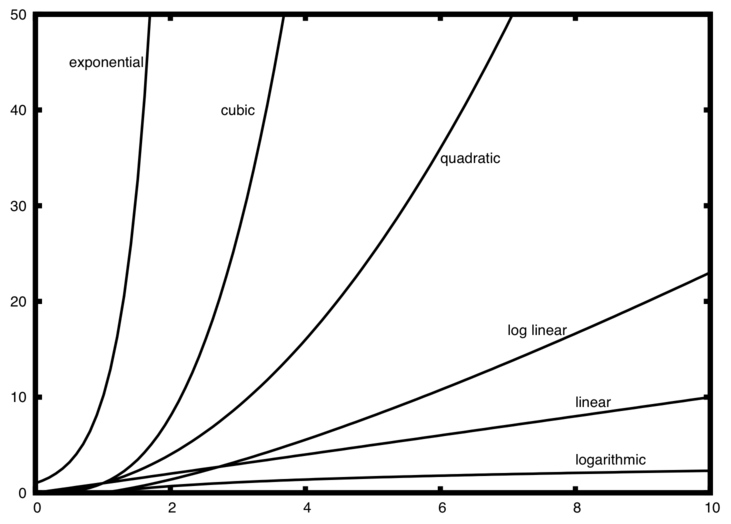
\includegraphics[width=4in]{images/newplot.png}
\end{figure}

\end{frame}

\begin{frame}\ft{\secname}

 观察以下程序,虽然它没有做任何事,但是对我们获取实际的代码和性能分析是有益的。
 \lstinputlisting{code/ex1.py}
 \pause

 $$T(n)=3+3n^2 +2n+1=3n^2 + 2n+4$$
\end{frame}


\begin{frame}\ft{\secname}
  
\begin{figure}[htbp]
        \centering
        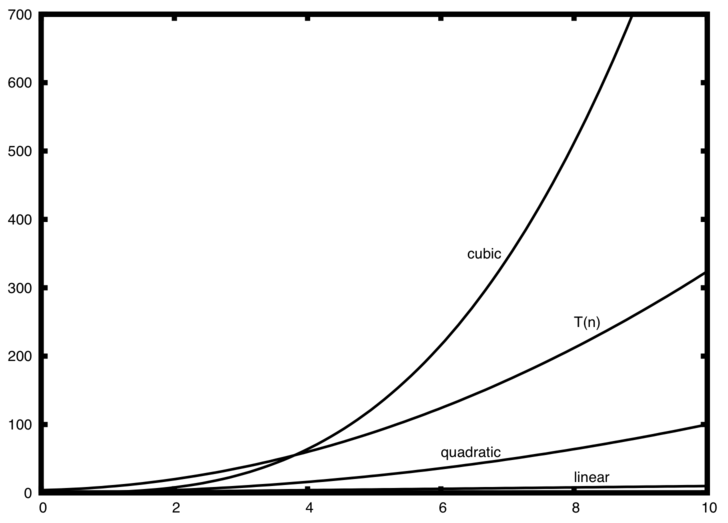
\includegraphics[width=3.5in]{images/newplot2.png}
\end{figure}
一开始,$T(n)$ 大于三次函数,后来随着 $n$ 的增长,三次函数超过了 $T(n)$。 $T(n)$ 随着二次函数继续增长。
\end{frame}

